% This is LLNCS.DEM the demonstration file of
% the LaTeX macro package from Springer-Verlag
% for Lecture Notes in Computer Science,
% version 2.4 for LaTeX2e as of 16. April 2010
%
\documentclass{llncs}
%

% Put edit comments in a really ugly standout display
\usepackage{xcolor} 
\usepackage{ifthen}
\usepackage{amssymb}
\usepackage{graphicx}
 
\newboolean{showcomments}
\setboolean{showcomments}{true} % toggle to show or hide comments
\ifthenelse{\boolean{showcomments}}
  {\newcommand{\nb}[2]{
    \fcolorbox{gray}{yellow}{\bfseries\sffamily\scriptsize#1}
    {$\blacktriangleright$#2$\blacktriangleleft$}
   }
   \newcommand{\version}{\emph{\scriptsize$-$working$-$}} 
  }
  {\newcommand{\nb}[2]{}
   \newcommand{\version}{} 
  }
 
\usepackage[linewidth=1pt]{mdframed}
\usepackage{lipsum} 

% for comments
\newcommand\levi[1]{\nb{Levi}{\textcolor{teal}{#1}}}
\newcommand\saadbin[1]{\nb{saadbin}{\textcolor{teal}{#1}}}
\newcommand\salman[1]{\nb{Salman}{\textcolor{blue}{#1}}}
\newcommand\vincent[1]{\nb{vincent}{\textcolor{red}{#1}}}
\newcommand\ralf[1]{\nb{ralf}{\textcolor{black}{#1}}}
\newcommand\ed[1]{\nb{ed}{\textcolor{green}{#1}}}

\usepackage{makeidx}  % allows for indexgeneration

\setlength{\textwidth}{13.5cm}
\setlength{\textheight}{20cm}
% \setlength{\oddsidemargin}{1.1cm}
% \setlength{\evensidemargin}{1.1cm}
%
\begin{document}
%
\frontmatter          % for the preliminaries

\mainmatter              % start of the contributions
%
\title{Process-Aware Model-Driven Development Environments}
%
\titlerunning{}  % abbreviated title (for running head)
%                                     also used for the TOC unless
%                                     \toctitle is used
%
\author{Levi L\'ucio\inst{1} \and Saad Bin Abid\inst{1}
 \and Salman Rahman\inst{1} \and Vincent
Aravantinos\inst{1}\and\\ Ralf Kuestner\inst{2}\and Eduard Harwardt\inst{2}}
%
\authorrunning{} % abbreviated author list (for running head)
%
%%%% list of authors for the TOC (use if author list has to be modified)
\tocauthor{}
%
\institute{
fortiss GmbH\\
\email{\{lucio,abid,aravantinos\}@fortiss.org,
salman.rahman@tum.de}\\
\and
Diehl Aerospace\\
\email{\{ralf.kuestner,eduard.harwardt\}@diehl.com}
}

\maketitle            
\begin{abstract}
\vspace{-.7cm}
Due to recent advances in Domain Specific Language (DSL) workbenches, it has
become possible to build model-driven development environments as sets of
individual DSLs that get composed for a specific purpose.
In this paper we explore how model-driven development environments can
become process-aware, to assist the user when building a model.
We offer an explanation to our ideas at three levels of abstraction:
1) the \emph{meta-meta} level, where brick DSLs are built using the
Meta-Programming System (MPS) workbench; 2) the \emph{meta} level, where brick
DSLs are assembled into frameworks that are further tailored for
particular modelling scenarios through the introduction of an explicit process
for model construction; and 3) the \emph{model} level, where
models are built through progressive tool-guided refinements and automated
steps based on the process introduced at the \emph{meta} level.
We exemplify our approach by providing the main highlights of the ongoing
development of a model-driven requirements gathering environment for our
industrial partners.
\vspace{-.7cm}
% The levels of abstr are illustrated: the individual brick languages for
% gathering requirements; how these DSLs are composed and organised to 
% fulfill our partner's requirements gathering process; and an example of using
% the system to build 
\end{abstract} 

\section{Introduction}
\label{sec:intro}
\vspace{-.3cm}
The current trends in domain specific software engineering, domain specific
languages (DSL) and domain specific modelling languages (DSML) demonstrate the
interest for \emph{tailored} software solutions.
When it comes to model-driven engineering (MDE) tools, studies like \cite{DBLP:conf/models/WhittleHRBH13} 
show that this trend is justified: among the MDE tools considered
in the reported study, the ones which were successful in penetrating industry
were precisely those which were developed in a tailored manner for a given
audience, the recommendation being: ``Match tools to people, not the other way
around''.

Many technologies now precisely enable this sort of tailoring, among which 
JetBrains' MPS \cite{DBLP:conf/pppj/PechSV13},
Xtext \cite{DBLP:conf/oopsla/EysholdtB10},
Sirius \cite{DBLP:conf/asplos/HauswaldLZLRKDM15}, or the classic MetaEdit+ \cite{DBLP:conf/sle/Tolvanen16}.
With the maturity of these technologies, one can safely say that building your own MDE tool
has never been so easy -- technology enthusiasts in various industries now
develop their own domain- or even company-specific tools.

On the other hand, as \cite{DBLP:conf/models/WhittleHRBH13} also mentions, tools
are an enabler, but they are not everything: ``More focus on processes, less on
tools".
Even when a tailored tool is available, allowing the modelling of one's domain
through many sub-DSLs makes it such that new users often become overwhelmed by
the amount of modelling techniques at their disposal. This is in fact the case
for even very specialized tools like Sfit \cite{DBLP:conf/vamos/BayhaLAMI16} for
the modelling of industrial manufacturing -- while modelling a restricted
domain, the tool contains a large number of different models, mostly rendered as
diagrams. The question of methodology or process then naturally follows: in
which order should one build the diagrams? More generally, which information
should one model at a given point in time? The funding of research projects
focusing on this question demonstrates the relevance of this question: for
example SPES-XT \cite{DBLP:books/sp/spes2016}, targets the development of
methodologies for the domain of embedded systems.
Similarly, Arcadia \cite{DBLP:conf/syscon/BonnetVEN16} emphasizes the importance
of the methodology in connection with MDE.

Just like for tools however, methodologies and processes can seldom be general
enough to match all use cases and answer all needs. There is thus also a need
for tailoring at that level. To facilitate the acceptance of the methodology, it
is essential that the tool \emph{supports} the methodology: this is for instance
the case with Capella and Arcadia.
Capella however, supports only the Arcadia methodology which is specific to
avionic systems engineering and to the processes of Thales.
All the above points to the fact that, if the tools can be tailored, the process
itself should be tailorable.

In this paper, we propose precisely an approach to develop DS(M)Ls in JetBrains'
MPS, \emph{equipped with a means to customize the tool in order to support a
given process:} using out approach, in addition to the usual MPS mechanisms to
develop their DSLs, developers can also explicitly express their own process.
Such a process of model construction is declared as a
statechart-like diagram, being that the current state is defined by the
satisfaction of some properties of the model as well as by its previous states.
For each state, the tool developer can define hints to be displayed as well as
quickfixes in the form of creation of new artifacts.

In order to clarify our work we draw an analogy with the M-levels defined by the Object Management Group:
\vspace{-.1cm}
\begin{itemize}
  \item M3: the MPS tool with its language definition capabilities.
  \item M2: development and composition of ``brick DSLs'' in a
  domain-specific model-driven development environment, together with a
  model construction process.
  \item M1: usage of the developed domain-specific tool.
\end{itemize}
\vspace{-.1cm}
We also identify four different \emph{roles} in the development and
usage of the framework:
\vspace{-.1cm}
\begin{itemize}
  \item the \emph{framework developer} (in our case JetBrains), who develop MPS
  (level M3),
  \item the \emph{framework customizer} (the authors of this paper), who develop
  a library for process-customizable DSLs (level M2),
  \item the \emph{(domain-specific) tool developer} 
    (typically a consultant or the in-house technology department of a company)
    who actually develops the domain-specific tool, making use of our libraries (level M2),
  \item and the \emph{user} (level M1).
\end{itemize}
\vspace{-.1cm}
In this work, we contribute a framework at level M2 to support the tool developer
in developing a \emph{process-aware} domain-specific tool.
At the M1 level, a ``dashboard'' allows the user to know permanently what is the
next step to achieve.

As a case study, we demonstrate how to use this framework for the
specific domain of requirements engineering: the step-by-step formalization of requirements is a common approach,
making it, therefore, an ideal candidate for the development of a process-aware tool.
For this purpose, we have implemented a set of DSLs supporting the MIRA
\cite{MIRA13} framework, a general approach for the stepwise formalization of requirements
focusing on quality assurance for requirements.

A \emph{tool developer} can use this set of DSLs as a basis for their
model-based development environment, by composing them with more specific DSLs
of their own design. She can also ``drive'' the user in her requirements
formalization process by implementing a process using our \textsf{Process} language.
We illustrate this approach by developing a requirements-engineering tool
specialized in the development of hardware cooling systems, inspired from a case
study from our industrial partners at Diehl Aerospace.

% The remainder of this paper is structured as follows.  In
% section~\ref{sec:metameta} we describe the MPS framework, which we use as the
% technological basis for all the results presented in this paper.
% Section~\ref{sec:meta} then describes our case study -- a set of languages and a
% process for the incremental gathering and refinement of requirements,
% specialized for hardware cooling systems. Then, in section~\ref{sec:model},
% we exemplify the construction of the requirements for a specific fan-based cooling system, using
% the previously defined languages and refinement process.
% Section~\ref{sec:implementation} lifts the veil over some of the implementation
% details of our work and section~\ref{sec:related_work} provides pointers to work
% in the literature that closely relates to the results we present here. Finally,
% section~\ref{sec:conclusion} presents a discussion of this research and 
% potential future work.

The remainder of this paper is structured as follows.  In
section~\ref{sec:metameta} we describe the MPS framework, which we use as the
technological basis for all the results presented in this paper.
Section~\ref{sec:meta} then describes our case study -- the construction of a
model-driven development environment for the incremental gathering and
refinement of requirements. Then, in section~\ref{sec:model}, we exemplify the
construction of the requirements using the environment described in the previous
section. Section~\ref{sec:related_work} provides pointers to work in the
literature that closely relates to the results we present here. Finally,
section~\ref{sec:conclusion} presents a discussion of our research and potential
future work.
\vspace{-.5cm}

 

\section{The \emph{metameta} Level: MPS: A Language Meta-Editor}
\label{sec:metameta}
\vspace{-.3cm}
The metameta level (M3, in MOF terms) is where the bricks for our approach are
built. These bricks consist of DSLs, defined in the MPS (Meta Programming
System)~\cite{mps} framework. MPS is a stable and industrially-proven
projectional meta-editor which provides edition capabilities at the meta-levels
needed for our approach: M2 and M1. It uniformly integrates language and editor
design capabilities, together with code generation tools and in-built
correct-by-construction techniques such as meta-model conformance, syntax
highlighting, auto-completion or type checking.
MPS is developed by JetBrains, which assumes the role of \emph{framework
developer}.
Throughout this paper we will often use vocabulary that is close to that used in
the MPS world in order to remain aligned with the technical aspects of our
work. In particular, the following terms are recurrently used in what follows:
\vspace{-.3cm}
\begin{itemize}
  \item \emph{Language}: an MPS language includes a metamodel, in the classical
  EMF sense. It additionally includes one or more editors for its metamodel,
  which provide concrete syntax.
  \item \emph{Concept}: the MPS equivalent of metamodel class.
  \item \emph{Concept / language instance}: concepts can be instantiated, in
  the same way metamodel classes can. We will also sometimes write
  \emph{language instance} to refer to an instance of the \emph{root} concept of
  an MPS language.
  \item \emph{Intentions}: actions attached to
  concepts of a language, available to the user. 
%   Those actions can be launched by the user when the
%   focus of the editor is on objects which are instances of those concepts.
  \item \emph{Language composition}:  Reference or containment relations can exist between instances of
  concepts of different languages, which is the primary language composition
  mechanism in MPS.
 Another composition mechanism is the MPS model, which can contain instances of
 concepts belonging to many languages.
 %which  provides an additional means for language composition.
\end{itemize}
\vspace{-.7cm}
% At this level we had to extend the existing MPS framework with languages to
% define \emph{flow} and a \emph{dashboard}. Additionally, we have provided
% extension points to give the user the possibility to define her own constraints
% that can be used to direct the flow of edition of the composed model.


\section{The \emph{meta} Level: Defining a Requirements Gathering Framework in
MPS}
\label{sec:meta}
\vspace{-.5cm}
\subsection{A Generic Requirements Gathering Framework}
\label{sec:generic_req_fram}
\vspace{-.3cm}
The case study requirements gathering framework we introduce here borrows its
structure from the Model-based Integrated Requirement Specification and Analysis (MIRA)
Framework~\cite{MIRA13}. The main parts of the MIRA framework are
as follows:
\vspace{-.1cm}
\begin{itemize}
  \item The \emph{system context} describes the relevant elements that belong
  to the context of the system being developed.
  \item The \emph{requirement list} documents the capabilities and limitations
  of the system under development.
  \item The \emph{trace link list} keeps the relations between the artefacts
  being defined.
  \item The \emph{QA} collection describes quality assurance activities and
  results.
\end{itemize}
\vspace{-.1cm}
This broad classification of the concepts necessary to build a requirements
gathering framework is helpful to us in a operational manner. We wish to build
our framework as a set of composed domain specific languages in the MPS
environment. For that we need an architecture around which we can organize such
languages. The MIRA architecture thus helps us in understanding how to group and
compose those languages. A particularity of MIRA is that \emph{quality
assurance} is natively integrated in the framework. MIRA's quality assurance
also has an operational counterpart in the MPS environment -- in terms of
language checks that come with the DSLs defined in MPS as well as other (formal)
analyses that can be defined by the \emph{domain-specific tool developer}
building the framework. These analyses are orchestrated during the definition of
the \emph{process} when building a tailored model-driven development environment
and correspond to MIRA's verification activities.\vspace{-.5cm}
\begin{figure*}[!h]
\centering
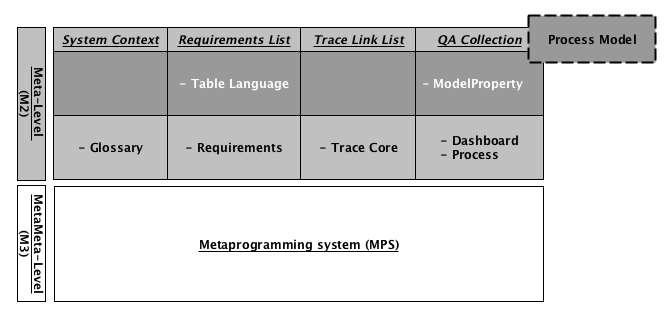
\includegraphics[width=.75\textwidth]{./figures/Fig2.png}
\caption{A language stack for gathering software requirements
}
\label{fig:meta_struct_reqs}
\vspace{-.7cm}
\end{figure*}
In figure~\ref{fig:meta_struct_reqs} we present the first two meta-levels of our
framework in the form of a stack of languages: at the bottom of the stack we
have MPS itself, with its meta-edition capabilities; in the layer immediately
above we define the four aspects of the MIRA framework. Each one of the four
aspects includes groups of DSLs that allow the requirements engineer to express
parts of the complete requirements model. The \emph{framework customizer}, in
this case our group at \emph{fortiss}, is responsible for building this part of
the stack. We have opted at this point for not including in the figure all the
DSLs that would be required to have a full-blown implementation of the MIRA
framework\footnote{The MIRA framework has been implemented as a requirement
specification plugin for the Autofocus environment~\cite{AF315}}, but rather the
following subset of those languages that is sufficient to exemplify our approach
in practice:
\vspace{-.2cm}
\begin{itemize}
  \item \emph{System Context}: this aspect of the framework contains a
  \emph{glossary language} to allow defining the domain specific glossary terms that are used across a
  requirements project, together with values associated to those
  terms.
  \item \emph{Requirements List}: this aspect of the framework contains a
  \textsf{Requirements} language for expressing textual requirements, together with meta-information
  such as the author of the requirement or the requirement's current state.
%   ; a \textsf{Component} language\levi{we don't actually use components in our
%   example} to describe how systems are descomposed in components and how those
%   components behave and interact with each other.
  \item \emph{Trace Links}: this group contains a generic \emph{trace
  language} that can be extended to building trace links from any to any model
  element in MPS.
  \item \emph{QA collection}: the QA collection group includes the
  \textsf{Process} and the \textsf{Dashboard} languages. The \textsf{Process}
  language allows defining which refinement tasks the requirements engineer.
%   needs to perform in order to build sound requirements. The reason that led us
%   to the inclusion of the \textsf{Process} language as part of the  \emph{QA
%   collection} aspect of the framework has to do with the fact that analyses of
%   the model are performed by our tool to allow calculating the current
%   state of the process of edition of the model. In our framework these analyses
%   include checks for soundness and completeness of the model, which correspond
%   to the verification tasks in MIRA.
  The \textsf{Process} language is used in conjunction with the
  \textsf{Dashboard} language in order to define at which moments a specialized requirements
  gathering framework will provide visual hints and press-button actions that
  guide the requirements engineer in the direction of achieving her task in a
  correct manner. Note that the \textsf{Process} language allows structuring a
  \emph{schedule}, or \emph{script} for building a complex model which relies on
  incrementally satisfying formal properties of the model. These formal
  properties are defined by the user or exist natively in MPS in the form of
  e.g. metamodel constraints or type checks.
%   Note that progressing through a particular flow of tasks is measured by the
%   success or failure of a set of automatic analyses. These analyses run on the
%   background of a specific requirements framework and will either need to
%   implement as part of a specific requirements gathering framework (at level
%   M1), or can already exist as part of the standard MPS analyses available for
%   the languages in the framework.
\end{itemize}
\vspace{-.5cm}
% Note that although we have used MIRA as a reference for our project work with
% our industrial partners, additional explanations on the framework are beyond the
% scope of this paper. We refer the interested reader to~\cite{MIRA13}.

% \begin{figure*}[!h]
% \centering
% 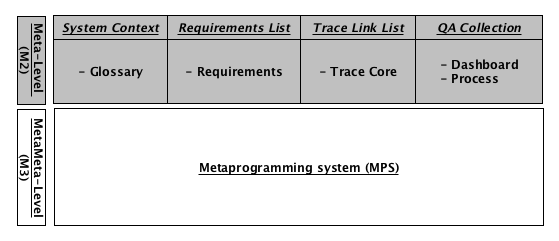
\includegraphics[width=.7\textwidth]{./figures/Fig1.png}
% \caption{A customizable language stack for gathering software requirements}
% \label{fig:meta_struct_reqs}
% \end{figure*}

\subsection{Customising the Framework: An Industrial Case
Study}
\label{sec:custom_frame}
\vspace{-.3cm}
Nowadays, many embedded hardware systems (e.g. in laptops, cars or planes) are
assembled together with cooling systems. The main purpose of those cooling
systems is to maintain an appropriate temperature during the operation of those
hardware electronics. In this section we will extend the generic requirements
gathering framework that has been introduced in
section~\ref{sec:generic_req_fram} in order to specialize it for gathering
requirements for software controllers for hardware cooling systems. In
particular, we will add a process for specifying this type of requirements.

The case study we present here is inspired by a requirements document (that for
non-disclosure reasons we cannot cite here) which was made available to us by
Diehl aerospace, one of our industrial partners. Diehl builds hardware for
airplanes and, as such, cooling systems for that hardware also need to be
produced. The process of gathering requirements the software that controls such
cooling systems is currently almost completely manually done. This poses a
problem to Diehl, as the current requirements gathering process imposes a large
amount of effort to ensure that those requirements are documented in a fashion
that is complete, correct and traceable. Additionally, the aerospace industry
has to adhere to strict regulations such that their systems can be certified to
be used in production. 
% Software reviewers require precise documentation for
% requirements, which is difficult to produce and maintain when little automation
% is available.
% The automation we present here is modelled as a set of tool-guided refinement
% steps, starting from abstract requirements and incrementally proceeding towards increasingly concrete ones. The idea behind the
% framework is that each refinement step will be done using an MPS language at the
% right level of abstraction. Constraints enforced by the such languages, together
% with analyses running on the background sheduled by a flow model will make sure
% that requirements are, to a large extent, well-formed by construction.\\

In order to specialize the language stack presented in
figure~\ref{fig:meta_struct_reqs} we have added the following languages: the
\textsf{Table} language, for defining the behavior of the controller for the
cooling system; the \textsf{ModelProperty} Language, which contains algorithms
implementing analyses of properties that are specific to the cooling system
requirements gathering system.
Additionally, the \emph{domain specific tool developer} also builds a process
that will configure the dashboard's behavior. The dashboard assists the
requirements engineer during the construction of the requirements by displaying
hints and press-button actions that guide the refinement of the requirements
model.

The dashboard is configured by a description of which hints should be
provided to the requirements engineer under which conditions. This information
is provided as an instance of the \textsf{Process} language.
In figure~\ref{fig:flow_statechart} we provide an example of such a process,
depicted as a statechart, for the	cooling controller requirements.  
The top part of each state in the figure includes the conditions that need to be satisfied such that the hint in the lower part of
that state is displayed on the dashboard. 

The conditions described on the statecharts' states are boolean properties that
are checked on the current state of a requirements project. These properties are
implemented in the \textsf{ModelProperty} Language in
figure~\ref{fig:meta_struct_reqs}. This language holds the algorithms that implements
the analyses required for our specific requirements gathering system.
Note that, although this customization work has been done at fortiss, the idea
is that in the future this work would be performed by a \emph{domain specific tool
developer} at Diehl. In a similar fashion, frameworks for gathering requirements for purposes
other than for cooling systems could also be customized using as basis the same
original set of languages as the one described in
section~\ref{sec:generic_req_fram}.
\vspace{-.7cm}

% Given they are
% specific to the cooling system requirements gathering framework, they are are
% defined at the model level of abstraction (M2), on top of the bare-bones
% requirements gathering framework.\levi{review levels of abstraction}

% Hints can be of two types: \emph{creational} or \emph{informational}.
% Creational hints enable the user to automatically generate new instances of
% languages in order to complete the model. On the other hand, informational hints
% serve as guidance steps to the user but are not associated with automatic
% actions. This means the requirements engineer has to manually perform a set of
% actions in order to further refine the requirements model and reach the next
% state of refinement of the requirements model as defined in the hint model in
% figure~\ref{fig:flow_statechart}. 

% Note that, when the hint is creational, the concepts that need to be created
% can also be declared together with any data that need to copied from the
% unrefined onto the refined model.

% The current dashboard allows the requirements engineer to perform a certain kind
% of analysis during the requirement construction. The analysis is implemented
% using the constraints.
% At present, the constraints are implemented for the individual models
% (requirement and table languages).

% The types of constraints implemented for performing the analysis are, 1) model
% properties constraints, 2) type-system constraints and 3) self-defined
% constraints.
% Examples of the analysis performed during the requirement construction is as
% follows,
% \begin{itemize}
%   \item If the Requirements model is empty or not
%   \item If the Glossary terms are defined in the requirements
%   \item If the values of the glossary terms (i.e., min/max) are set in the
%   Glossary model
%   \item If the parts of the Requirement model are completely defined or not
%   \item If the cooling function increasing/decreasing intervals are continuous
%   \item If the values of increasing and decreasing intervals are between the
%   preset min and max thresholds
% \end{itemize}


% During the requirement construction process the requirements engineer is guided
% by a set of hints. The implemented hints can be categorized as follows, 1) the creational hints and 2) the informational hints.
% Creational hints enables the user to perform actions automatically (e.g.,
% creating a new language instance) to complete the model. Whereas, the informational hint only
% serves as a guidance step to the user that is not associated with any
% action to be executed automatically. When an informational hint is provided to
% the user in the dashboard, the user has to manually perform the action in order
% to complete the requirement and resolve any errors. These errors in the
% requirement are caused because of the failed constraints
% discussed earlier.\saad{drafted}

% For clarity reasons, let us now briefly explain the process model depicted in
% figure~\ref{fig:flow_statechart}\levi{attach this text to a different picture}.
% The requirements engineer is initially provided with an empty dashboard with a creational hint to start constructing
% the requirements for the cooling controller.
% At this point an empty requirements project can be automatically built using the
% creational hint. An informational hint is then provided to guide the
% requirements engineer through defining the threshold values as glossary terms in
% the requirement and/or complete the requirements with all necessary data.
% Upon successfully building a requirement and defining the glossary terms, the
% requirements engineer is provided with a creational hint to perform the
% refinement step from a requirement and its threshold values into a cooling
% function describing the behavior of the controller.
% An empty cooling function (i.e., a model of the \textsf{Table} language) is then
% automatically created with the minimum and maximum thresholds values coming from
% the glossary terms. The user is then provided with feedback from the
% \textsf{Table} language until a correct cooling function is defined.

% at which
% point the user is provided with an informational hint that this part of the
% requirements is finished.

% \begin{figure*}[!h]
% \centering
% 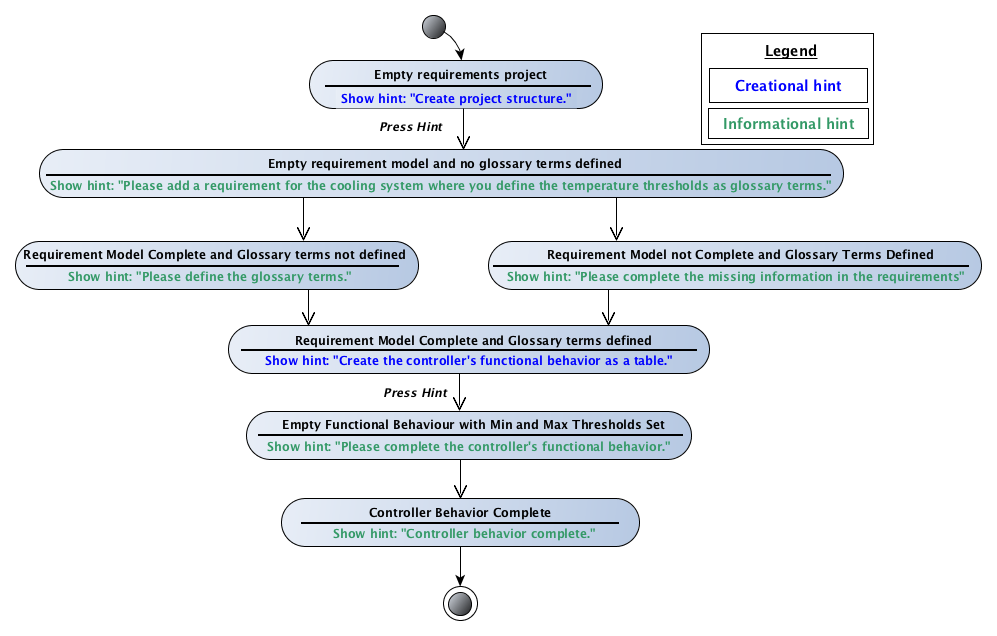
\includegraphics[width=.9\textwidth]{./figures/FlowChart_V2.png}
% \caption{A statechart-like representation of an instance of the \textsf{Flow}
% language}
% \label{fig:flow_statechart}
% \end{figure*}

% Note that the \emph{flow} language example in figure~\ref{fig:flow_statechart} is
% only an example of a possible flow. Arbitrary flows for describing any
% requirements gathering framework can be defined, built on top of also arbitrary
% boolean property checks defined in the \emph{custom analysis} language.

% There exits some limitations in the current implementation of the
% dashboard that are as follows,
% \begin{itemize}
%   \item for now the dashboard content and the hints are hardcoded in the
%   dashboard language
%   \item the dashboard should be an independent language, to be extended with
%   the holding specific models in the particular project.
%    \item a hint language for the flow can be defined as a statechart. Such
%    models would then need to be compiled (using an intention) to produce the
%    necessary transform actions in the dashboard language. The Dashboard language
%    should then be recompiled after the intention to generate the transform
%    actions is ran.
%    \item In the current version of the dashboard there are boolean constraints implemented. An example
% of a boolean constraint is to check if a particular property of a model is set
% or not (e.g., type of a requirement is set or not). At present we require more
% complex checking
%   \item Constraints are defined as methods in a separate language over the
%   languages on top of which the analysis should be defined.\saad{limitations
%   are our next steps. can be put in the future work section of the paper}
%       \end{itemize}

% MIRA aims at improving the quality of system under development by
% supporting quality assurance (QA).  At this level we had to extend the existing MPS framework with languages
% to define \emph{flow} and a \emph{dashboard} (although hard-code extensions would
% be the way to go for the future).
% 
% % The MIRA framework has been implemented as a
% % requirement specification plugin for the Autofocus environment~\cite{AF315}. In
% % particular, under the AF3 environment the MIRA framework provides an integrated
% % envrionment for building and formalizing the requirements for a particular
% % system under development.
% 
% At the meta level the framework to build the composed models for requirements is
% assembled. This framework consists of:
% 
% \begin{itemize}
%   \item A set of brick languages defined using MPS' metametalevel.
%   \item A set of constraints that extend the extension points defined at the
%   metametalevel.
%   \item A set of action hints associated to the constraints.
%   \item Levels of priority of satisfaction of constraints. A level includes a
%   set of constraints and a level is accomplished when all the constraints are
%   satisfied. Satisfying a sequence of levels will lead to the desired
%   composed model (analogy with gamification). Special attention has to be paid
%   to when checks have been satisfied but then stop being so. A statemachine
%   associated to the levels of priority should be kept updated as the composed
%   model gets updated by the user.
% \end{itemize}
% 
% 
% Our tool/dashboard is a guiding system that uses the
% requirements model along with some glossary terms (e.g., min/max values for the
% cooling system) for requirement construction. It also enables the user to
% perform refinements of the constructed requirement into an expected behavioral function (e.g., cooling
% function in our case study). These refinements are configured as a flow model
% implemented by a set of hints that are associated with the constraints.
% The flow model is implemented through a set of hints in our built
% tool/dashboard. \saad{text moved from model level}
% Additionally, we have provided extension points to give the user the possibility to define her own constraints
% that can be used to direct the flow of edition of the composed model.
% 
% \begin{itemize}
%   \item the Diehl case study
%   \item composing languages through traceability (and just MPS inclusion)
%   \item following Sabine's notion of requirements quality and instantiating MIRA
%   (using domain-level (inter-language) checks)
%   \item define a completion dashboard to guide the user through
%   formalizing requirements
% \end{itemize}

% \begin{figure*}[!h]
% \centering
% 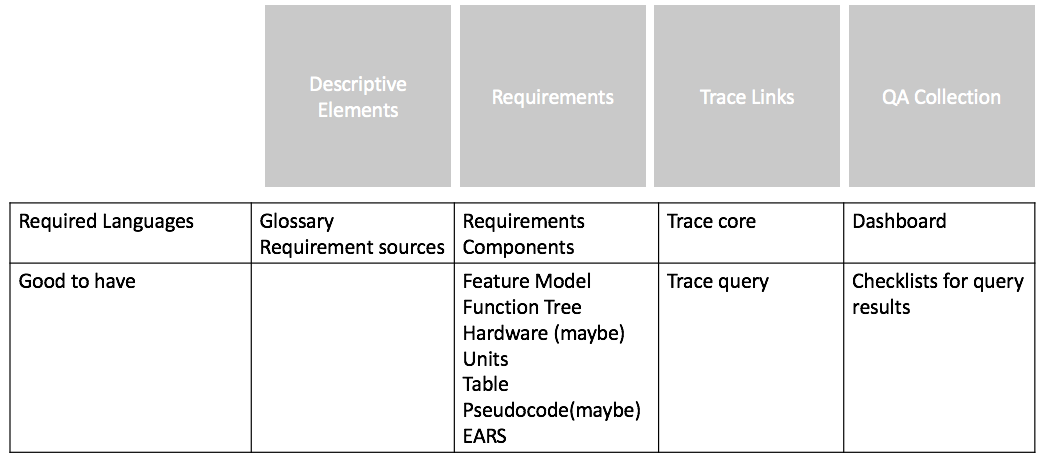
\includegraphics[width=\textwidth]{./figures/core_languages.png}
% \caption{Meta-structure for the definition of requirements gathering
% frameworks}
% \label{fig:meta_struct_reqs}
% \end{figure*} 

\section{The \emph{Model} Level: A Domain-Specific Requirements Gathering
Framework in Action}
\label{sec:model}
\vspace{-.2cm}
We will now exemplify how a user, in this case a \emph{requirements engineer},
can make use of the specialized requirements framework we have defined in section~\ref{sec:custom_frame}.
In particular, based on an existing requirements document provided by Diehl
Aerospace and following the directions made available to us from engineers at
Diehl, we will incrementally build the requirements for the software that
controls a fan-based cooling system to cool down hardware boards embedded in
the doors of passenger airplanes.
Because of the fact that airplane doors include slides that should only be
deployed when a plane lands under specific conditions, the logic running in
those boards is non-trivial. The goal of the controller is to make
sure the cooling fan runs at the correct duty cycle (fan speed) such that the 
hardware board works under ideal temperature conditions. The calculation of
the duty cycle for the fan at a given time depends on two inputs:
1) the current temperature of the hardware board that needs cooling; and 2)
whether the hardware board's temperature is increasing or decreasing.
 
% In the text that follows we will describe how to build the requirements for the
% fan controller software using the framework defined in section~\ref{sec:model}.
% This will be achieved by starting from an abstract requirement containing only a
% natural-language description of the fan's operation, and then performing a
% set of tool-guided and tool-supported refinements that in the end lead to a description
% of the expected behavior of the fan cooling system as a function.

Note that in the example that follows we do not pretend to be exhaustive in the
construction of the requirements for the fan's controller. This section
reflects part of our partners' requirements refinements process and demonstrates
our framework's abilities in terms of providing automated assistance to the
requirements engineer. 
\vspace{-.3cm}
\subsection*{Tool Supported Requirements Definition and Refinement}
\vspace{-.1cm}
The first thing to do in a requirements project for a cooling controller is to
create a new dashboard by instantiating the \textsf{Dashboard} language that
implements the cooling controller requirements process. A newly generated
dashboard for our fan requirements project is depicted in
figure~\ref{fig:empty_dashboard}.
The dashboard is the central artefact the requirements engineer refers to during
requirements construction. It displays the current hint given to the
\emph{user}, as well as the current state of the requirements refinement process
as a graph or a table. The hint displayed by the dashboard at the beginning of
the project is ``Create Project Structure''. This hint is creational, which
means the \emph{user} can mouse-click on the hint to produce the instances of
concepts that constitute the initial structure of the project in the same model
where the dashboard instance has been created. Following this action a new hint,
as shown in figure~\ref{fig:dashboard_newreq}, proposes to the requirements
engineer defining a new requirement for the system that includes the temperature
thresholds for the functioning of the cooling system.
Note that at this point the current state of the requirements model has now
changed to ``Empty requirements model and no glossary terms defined'', as
highlighted in orange in figure~\ref{fig:dashboard_newreq} -- which now presents
a tabular view of the refinement process.
\vspace{-.6cm}
\begin{figure*}[!h]
\centering 
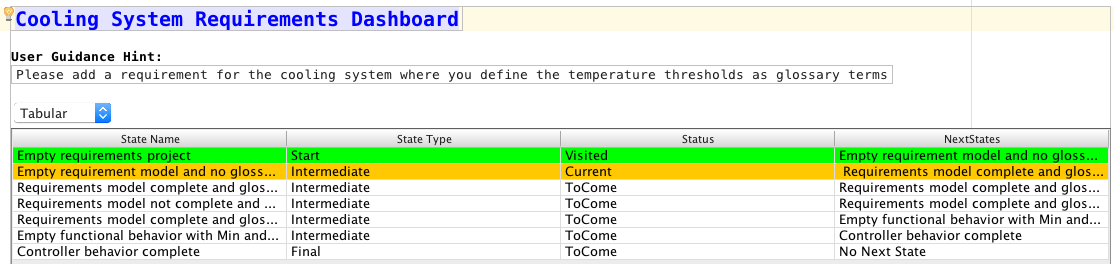
\includegraphics[width=1\textwidth]{./figures/DefineCoolingReq.png}
\vspace{-.7cm}
\caption{The Dashboard provides a hint for adding a new requirement}
\label{fig:dashboard_newreq}
\vspace{-.7cm}
\end{figure*}

The overall desired behavior of the cooling controller is stated as is an instance of the
\textsf{Requirements} language in figure~\ref{fig:new_req}. From this
requirement the requirements engineer can then extract minimum (e.g., ``Minimum
increase value') and maximum (e.g., ``maximum increase value') threshold values
using the MPS intention ``Extract Into Glossary''. When used, this MPS intention generates in the project's glossary an entry with the same names as words or sets of words
selected from the text. This constitutes the first
refinement of the original abstract requirement. The next step is to define the duty cycle of the fan as a function of the current temperature of the controller board and whether the temperature is going up or down. The dashboard assists the requirements engineer in this task by
providing a hint that, when mouse-clicked, automatically generates a table to
define such behavior. An example of such a table is depicted in
figure~\ref{fig:FAU_behavior_2d}.
% ``\emph{The cooling controller shall cool down the hardware board by adjusting
% the speed of the fan to an appropriate duty cycle. The duty cycle depends on the
% current temperature of the hardware and whether that temperature is increasing
% between a minimum increase value and a maximum increase value, or decreasing
% between a maximum decrease value and a minimum decrease value.}''\\
 \vspace{-.5cm}
\begin{figure*}[!h]
\centering 
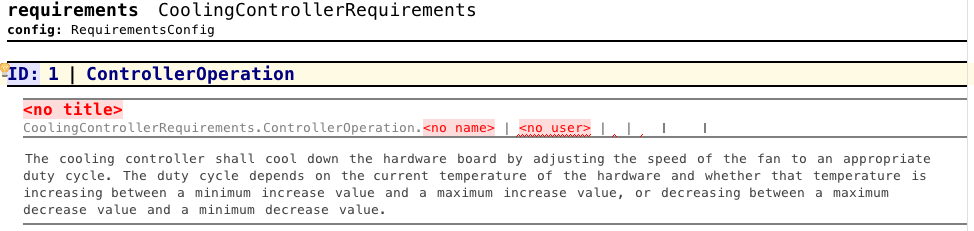
\includegraphics[width=1\textwidth]{./figures/textReqIncomplete.png}
\vspace{-.7cm}
\caption{The requirements engineer adds a new requirement}
\label{fig:new_req}
\vspace{-.7cm}
\end{figure*}

% \begin{figure}[!h]
% \centering 
% 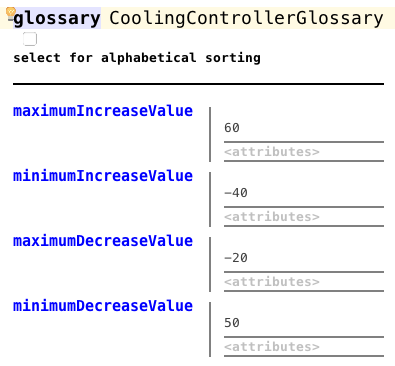
\includegraphics[width=.7\textwidth]{./figures/glossary.png}
% \caption{The glossary for the cooling controller requirements}
% \label{fig:glossary}
% \end{figure}
% Although the glossary terms for the temperature thresholds have now been
% defined, the requirement itself is still not complete, as shown by the
% dashboard's hint in figure~\ref{fig:error_dash}. This situation can be further
% investigated in detail by applying the MPS intention ``Create Error Dashboard''
% on the dashboard. In figure~\ref{fig:error_dash} a console error view
% with information about which model element currently contain which errors helps
% the user in identifying and fixing the remaining errors.
% 
% \begin{figure*}[!h]
% \centering 
% 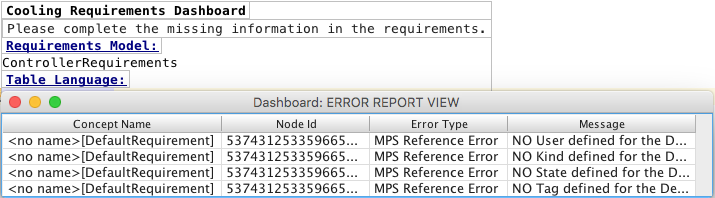
\includegraphics[width=1.7\columnwidth]{./figures/ErrorDashboard.png}
% \caption{Detailed explanation of the errors in a model}
% \label{fig:error_dash}
% \end{figure*}
% \begin{figure*}[!h] 
% \centering 
% 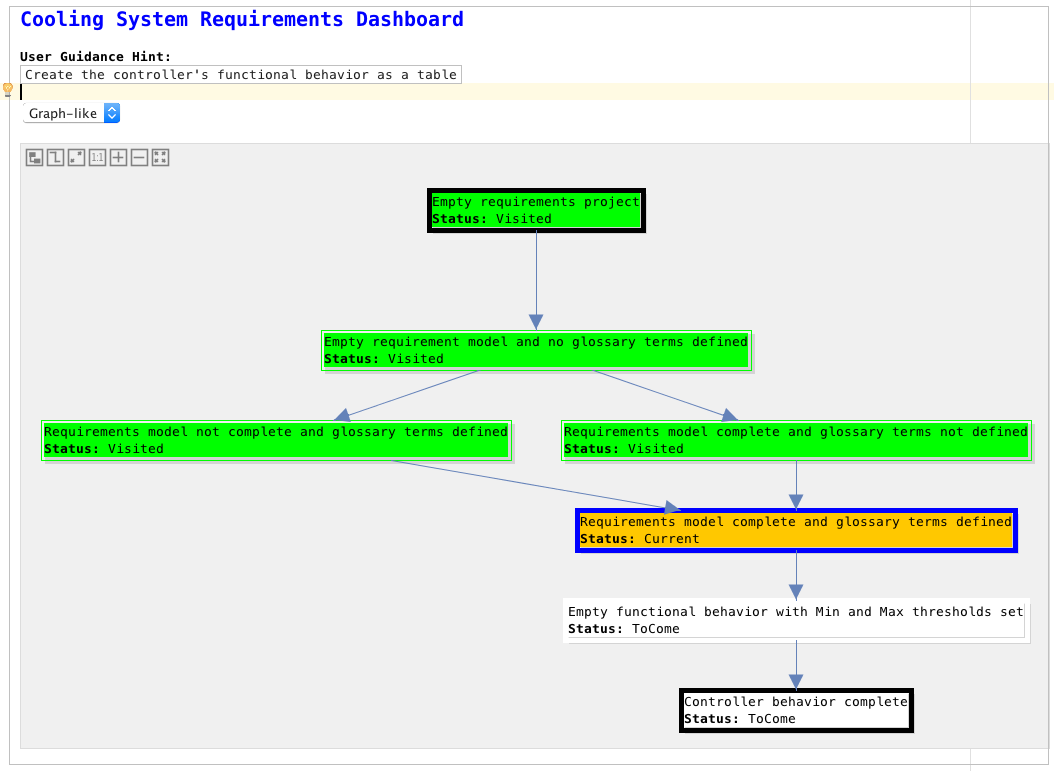
\includegraphics[width=1\textwidth]{./figures/CreateTable.png}
% \caption{The dashboard proposes creating a table to define the behavior of the
% fan controller}
% \label{fig:FAU_behavior}
% \end{figure*}
\begin{figure*}[!h]
\centering
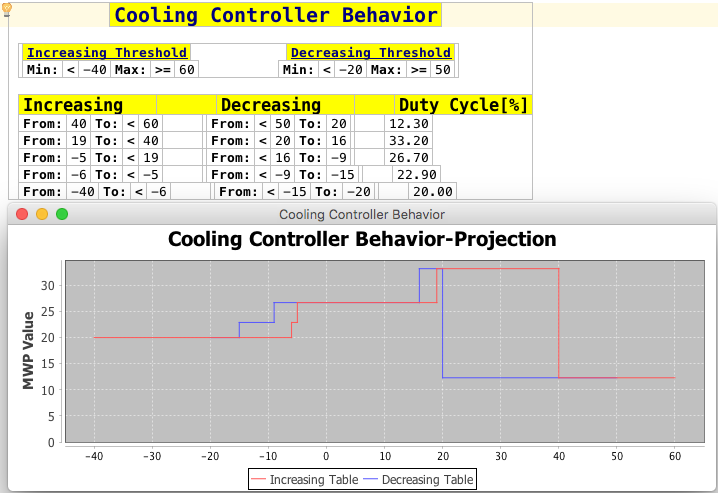
\includegraphics[width=.6\textwidth]{./figures/DiehlTableAnd2DGraph.png}
\vspace{-.3cm}
\caption{A filled in table and associated 2D visualization of the defined
function} 
\label{fig:FAU_behavior_2d}
 \vspace{-.7cm}
\end{figure*}
Note that the minimum and maximum threshold values in the table are preset in
advance, as the process itself defines they should copied from the values
previously stored in the glossary.
We now come to the last refinement, which is to precisely define the behavior of
the cooling fan's controller. In order to do this it is necessary to manually
insert rows in the table that define the duty cycle for given intervals of
temperature, when the temperature is going up or down.
% \begin{figure}[!h]
% \centering 
% 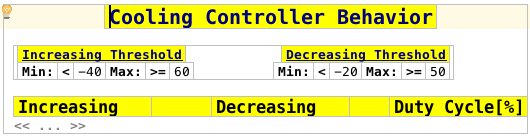
\includegraphics[width=1\textwidth]{./figures/DiehlTable.png}
% \caption{An empty table with filled in threshold values}
% \label{fig:FAU_behavior_thresh}
% \end{figure}
The \textsf{Table} language itself implements checks for completeness (all the
temperatures between the thresholds are mapped onto duty cycles) and
functionality (only one duty cycle value is given per temperature). Violations
of these properties are pointed out in the editor as red markers.
Figure~\ref{fig:FAU_behavior_2d} represents a filled in table holding, for
non-disclosure reasons, a fictitious behavior of the fan's controller.
In the figure a 2D-graph representation of the table is also visible and it is
produced by applying the “Visualize Graph” MPS intention to the table.
% \saad{Text moved from model level to instance level} Our example case study
%  is inspired by one of our industrial partners (i.e., Diehl aerospace) that builds cooling systems for airplane hardware. We have abstracted an example requirement, where the user is required to correctly build requirements leading to a description of the expected behavior of a cooling system. The abstract requirement that requires to be built and refined by the user contains the following,
% \begin{itemize}
%   \item the minimum and the maximum temperature thresholds of the controller
%   boards,
%   \item the behavior of the cooling system that it increases or decreases the
%   duty cycle of the cooling unit based on the current temperature of the
%   controller board and
%  \item whether the temperature is increasing or decreasing. 
% \end{itemize}

The running example we have described in this paper can be downloaded
at~\cite{coolingControllerProcess} as an MPS project. Another case study of
using our framework is available at~\cite{earsctrlProcess}, where we have
designed a process to assist the user in building natural langage-like
requirements for embedded controllers. Two videos demonstrating our
tool and portraying these two case studies can be found
at~\cite{coolingControllerProcessVideo,earsctrlProcessVideo}.
 \vspace{-.4cm}
  





%\section{A Peek into the Implementation Details}
\label{sec:implementation}

As previously mentioned, the framework we present here relies on the one hand on
DSL composition, and on the other hand on a process to guide the user through
the construction of a model. The most important blocks for defining a
process are \emph{properties} of the composed model being defined. These
properties extend an internal MPS Java \textsf{BaseLanguage} interface (defined
at the metameta M3 level), called \textsf{SpecificChecker}.
The  \textsf{SpecificChecker} interface is implemented by all model checkers
inside MPS. A few model checkers are already implemented inside MPS for
analyzing models and returning error instances. Those model checkers
search for example for typing errors or metamodel constraint violations. We
extend the same \textsf{SpecificChecker} interface in order to build our custom checkers that
can perform arbitrary checks on models, including interfacing with external
analyzers. We then wrap such checkers using concepts of the \textsf{Property}
language (see figure~\ref{fig:model_reqs}) to build the \emph{properties} which
are in turn used by the processes defined as instances of the \textsf{Process}
language.

The \emph{domain specific tool developer} is responsible for configuring the
process that will be used by the dashboard to provide hints to the final user.
This process is built as a instance of the \textsf{Process} language. An example
of such an instance can be observed in figure~\ref{fig:flow_model}, including the
first two states of the process for gathering requirements for cooling
controllers.

\begin{figure*}[!h]
\centering 
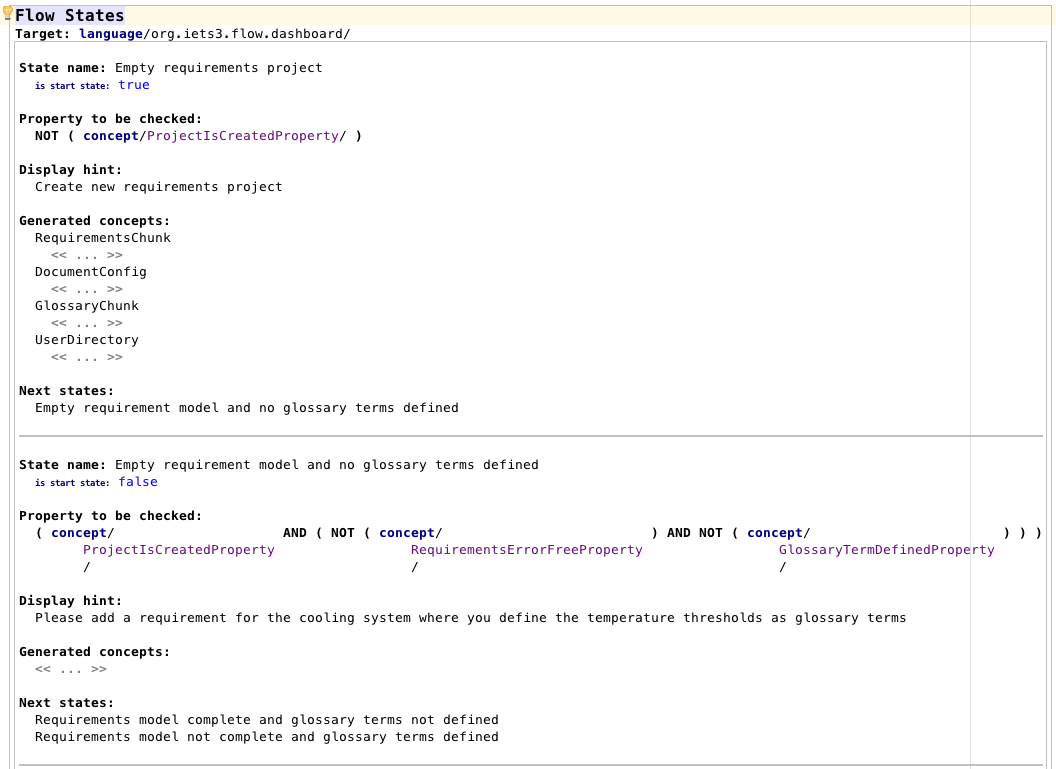
\includegraphics[width=1.55\columnwidth]{./figures/FlowModel.png}
\caption{An sample of the instance of the Flow language for the cooling
controller example}
\label{fig:flow_model}
\end{figure*}

A process model contains states, where for each state the  \emph{domain
specific tool developer} needs to define the type of state (\emph{start},
\emph{intermediate} or \emph{final}), its name, the \emph{condition} to be
checked on the model, the text that should be displayed in the hint box on the
dashboard, the new instances of concepts to be generated, if any, and the next
states. The \emph{condition} of a state is built as a propositional logic
formula having as propositions concepts of the \textsf{Property} language, that are to
be checked on the requirements model. Note that it is also possible to declare in a process
state that data is copied from existing parts of the model onto the new
instances that are created in case the hint is \emph{creational}.

Once a process as been defined, the \emph{domain specific tool developer} can
then use an MPS intention to copy the process data in
figure~\ref{fig:flow_model} to the \textsf{Dashboard} language declared as the
\emph{target} at the top of figure~\ref{fig:flow_model}. This makes it such that
the \textsf{Dashboard} language becomes aware of the process to be used for the
model-driven development environment being built.

When a new dashboard is created in a project as an instance of the
\textsf{Dashboard} language, an algorithm will continuously run in the
background for calculating the current state of the process of creation of the composed model.
This algorithm relies on the fact that the process graph has the following
properties: it is a directed acyclic graph, having only one \emph{start state}
and one \emph{end state}. Additionally, we also assume that forks imply
different paths to achieve the same goal. This is enforced by mutually
exclusive conditions on the  states that follow a fork. As an example, in
figure~\ref{fig:flow_statechart} it can be seen that the requirements model can be completed before the glossary terms are introduced, or
the other way around. However, both must be finished before the ``Requirements
Model Complete and Glossary Defined'' state. A corollary of this assumption 
is that only one state at a time can be the current state in the process
graph flow.

The algorithm that calculates the current state operates by starting at the
initial state and following the flow model graph until no more states can be
found that satisfy the model. The last state that satisfies the model is
returned as the current state. By skipping intermediate states that evaluate to
\emph{true} we avoid stopping the search at states of the process which will
always be satisfied by the composed model after a given point, such as the
``Requirement Model Complete and Glossary Terms Defined'' state in our running
example.
% Note that this algorithm accomodates the fact that properties stated in already
% visited states in the process may evaluate to \emph{false} once the user
% advances in the construction of the composed model. An example of one of such
% conditions is the formula for the ``Empty requirements project'' state in figure~\ref{fig:flow_model}, which is the
% negation of the property that the project exists. Naturally, once the project is
% created this condition will become \emph{false}. When searching for the
% current state, the algorithm skips states that evaluate to \emph{false}.

The main advantage of this algorithm we present here is that it allows for the
current state to go backwards if parts of the model are deleted, as the process
is always searched from the start. However, given our semantics of always
returning for the latest state which property is satisfied by the model, care
should be taken when designing the conditions on states. In particular,
deletions in the model should not lead to inconsistencies between the current
state as reported by the dashboard and the real current state.\levi{talk about
extrapolating the algorithm to multiple end states and multiple current states}

The running example we have described in this paper can be downloaded
at~\cite{coolingControllerProcess} as an MPS project. Another case study of
using our framework is available at~\cite{earsctrlProcess}, where we have
designed a process to assist the user in building natural langage-like
requirements for embedded controllers. This second case study is based on the
work we have previously implemented on the EARS-CTRL tool~\cite{NFM17} and it
features properties in the process definition that are analysed by interfacing
with the  external~\textsf{autoCode4}~\cite{autoCode17} tool. Note that
both~\cite{coolingControllerProcess,earsctrlProcess} are GitHub repositories
that contain not only MPS projects, but also additional information about how to
install those projects as well and pointers to videos demonstrating the usage of
our framework.

% DSL composition is achieved using MPS' native
% mechanisms where references to objects of a DSL can simply be embedded in
% objects of another DSL. This can be observed for example in
% figure~\ref{fig:new_req}, where the ``RequirementsConfig'' object that
% defines some metadata for the project is refered to from an object where a
% requirement is defined.


\vspace{-.1cm}
\section{Related Work}
\label{sec:related_work}
 \vspace{-.4cm}
Mechanisms for providing some kind of guidance to the domain-specific
language user are present, to a smaller or larger extent, in all DSL definition
workbenches. In most cases, that guidance is provided in the form of
correctness-by-construction (e.g. only correct models that conform to a
metamodel can be built), or a-posteriori checks for conformance to certain
well-formedness rules. This is the case for example for DSL workbenches such as
Sirius~\cite{DBLP:conf/asplos/HauswaldLZLRKDM15}, AutoFocus3~\cite{AF315},
MetaEdit+\cite{DBLP:conf/sle/Tolvanen16} or MPS~\cite{DBLP:conf/pppj/PechSV13}
itself. However, none of those tools is capable of natively providing the means
to explicitely define a model construction process or methodology that can
assist users when building instances of DSLs specified in those environments.

Model construction processes naturally depend on the domain the DSLs are aimed
at. It is thus not surprising that the explicit notion of process is more
present in modelling environments that are specifically aimed at certain domains
-- as previously mentioned, the Capella tool is a model-driven engineering
solution for systems and software architecture engineering which enforces the
Arcadia~\cite{DBLP:conf/syscon/BonnetVEN16} methodology, aimed at specific
domains such as transportation, avionics, space or radar; the Soley tool
suite~\cite{soley}, dedicated to model-based data extraction, processing and
visualization, includes workflows as first-class citizens.
% Workflows are sequences of model transformations leading to analysis results
% that can be played (semi-)automatically, as well as recorded by the tool from a
% set of user actions.

Coming back to generic workbenches for language constructions, there exists a
large body of work in the area of model transformation chaining to orchestrate
the flow of models to achieve a modelling goal. For example, authors such as
Wagelaar~\cite{wagelaar2006blackbox}  or Kolovos~\cite{Kolovos2008} propose
mechanisms for automatically orchestrating model transformations such that
certain modelling goals are achieved. In this area, the study which is the
closest to the proposal in this paper is the FTG+PM
framework~\cite{DBLP:conf/sdl/LucioMDVJ13,MustafizDLV12}. The FTG+PM defines an
explicit process for the execution of model transformations.
Enacting that process means that certain model transformations are performed
automatically, while for others the user will have to input data at given
points. The differences with the work we present in this paper have to do with
the fact that our process is non-invasive, and is aimed at advising the user
rather than executing a pre-defined work flow. With our approach automated
actions are proposed to the user, who remains in complete control of the model
edition process at all times.

% Note although mechanisms like the one we propose in this paper do not exist in
% DSL workbenches such Sirius or AF3, it is possible to code them by using those
% workbenches' APIs and making usage of already existing analysis structures, as
% we have done for the work we present here. One of the differences that we are
% aware of regarding the AF3 workbench in particular, is that the guidance
% mechanism we present in this paper has been fully implemented using MPSs native
% mechanisms. Buiding the same mechanism in AF3 requires on the other hand
% extending the workbench's core framework using Java.
 \vspace{-.6cm}



\section{Conclusions and Future Work}
\label{sec:conclusion}
 \vspace{-.6cm}
We have presented a technique for the construction of
domain-specific model editors in MPS, where these editors are based on
a set of composed DSLs and on a description of the process that
should be followed when building the models for that domain. We have applied our
approach to the construction of an editor for gathering software requirements
at two levels: firstly, we build an abstract requirements gathering framework,
following the guidelines in the MIRA framework~\cite{MIRA13}; secondly, we
specialize that framework for our industrial partners at Diehl, by introducing
a specific requirements refinement process for controllers for cooling systems.

The main technical contribution of this paper are the means to define a process
to assist in building a model in a domain-specific model-driven development
framework. This process is based on a set of model analyses running in the
background of the framework and can guide the user until the model is complete.
At a methodological level, our contribution regards our ideas on the separation
of the \emph{framework customizer} and the  \emph{domain specific tool
developer} roles. While the former is responsible for defining a number of
fundamental ``brick'' DSLs, the latter further specializes them for a particular
application by potentially adding more languages and organizing the whole
according to a process.

In its current state, the main shortcoming of the technique we propose in this
paper is the fact that it is the complete responsibility of the domain-specific
tool developer to check the consistency of the properties being checked during
the unfolding of the process, as well as their logical sequence in the process.
Additional assistance during this step could be envisaged, for example in the
form of automated checks for logical inconsistencies in the conditions that
define each state in the process. Also, arbitrary deletions in the model may
lead to inconsistencies in the current state of edition in the dashboard. A
carefully designed process may avoid such inconsistencies, although automated
help for the tool developer would also be important here. Finally, scalability
is also an issue as analyses currently run very often in the background,
which will rapidly lead to performance degradation in larger systems. Potential
solutions to this problem are currently being investigated by colleagues of our
at fortiss~\cite{Models17Sudeep}.

As future work, beyond mitigating the shortcomings identified above, we will
work continue working with Diehl Aerospace to further develop the case study we
present in this paper into a usable requirements gathering system. Other partner companies
have shown interest in applying the work we present to domains other than
requirements engineering, which means in the future building or assembling
different language stacks as well as different processes. Closer integration
with MPS is necessary in order to perform analyses in the background only when
strictly needed. Finally, mechanisms for the systematic creation of standalone
editors that implement process-aware model-driven development environments
is also in our future plans.
 \vspace{-.6cm}
 

\section*{Acknowledgements}
The work presented in this paper was developed for the ``IETS3'' project, funded
by the German Federal Ministry of Education and Research under code
01IS15037A/B.
 \vspace{-0cm}
%\newpage

\bibliographystyle{plain}
\bibliography{bibliography}

\end{document}
